\label{ch:impl}
This chapter provides a detailed description of suggested abstraction of the AHB architecture. First the existing hardware is described in section \ref{sec:exist} followed by the necessary interfaces described in section \ref{sec:intfc}. The Gap Free Verification process was employed on the existing design to investigate what a feasible abstraction would be. This convoluted process required a few choices affecting the abstraction level and suggest an addition to SystemC-PPA. This is all covered in detail in section \ref{sec:syslev}. The end result is a an AHB described in SystemC-PPA which can perform up to 32-bit single reads and writes with some added latency. The ESL and RTL descriptions can be automatically generated for up to 15 master and slaves, together with properties proving that the ESL is a sound abstraction of the RTL. The choice of arbitration policy leads to situations where the notion of starvation comes into play, which is described in section \ref{sec:simulation}. Finally the inner workings of the generator is described in section \ref{sec:generator}. (I should highlight both here and in the introduction that this is a multi master design and that complicates the shit out of things)

\newpage
\section{Hardware overview}
\label{sec:hardover}
\begin{figure}[hbt]
    \begin{center}
        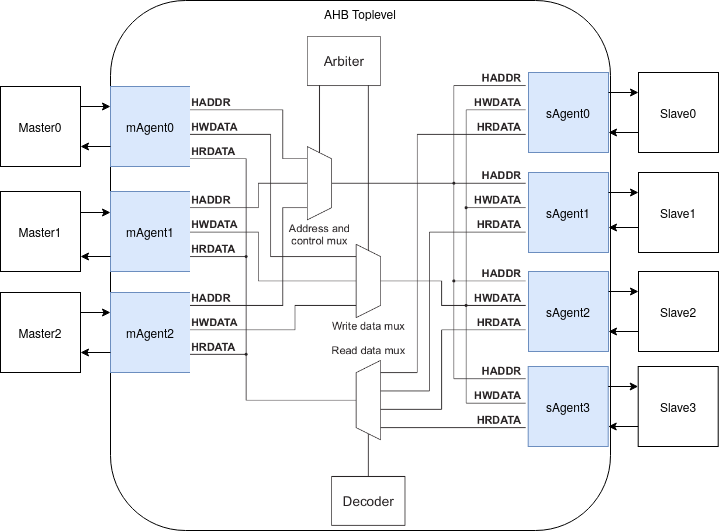
\includegraphics[width=0.8\textwidth]{figs/hw/Hw_toplevel.png}
    \end{center}
    \caption{Hardware toplevel with 3 masters and 3 slaves connected}
    \label{fig:hw_toplev}
\end{figure}

\subsection{Existing hardware}
\label{sec:exist}
The existing hardware is a stripped and slighlty modified version of the ahb system generator \cite{ahbsys}. Only the modules concerning the arbiter, decoder and interconnect are taken from this design. This architecture is a well recognized implementation of the AHB which follows the protocol. The implementation of an arbiter and interconnect in VHDL which properly follow the protocol is a complicated task. For the purpose of this thesis it was better to use existing hardware to avoid the need of reinventing the wheel, and the chosen implementation seem to be regarded as the best. Furthermore, its surrounding modules provides much insight into how AHB masters and slaves are implemented. This hardware model is the interconnect between the master and slave agents in figure \ref{fig:hw_toplev} including arbiter and decoder. This block is from here on referred to as the AHB matrix.

\subsubsection{Modifications}
One simple modification is made on this design. The original design provided a constant error signal on \textbf{HRESP} regardless of encoding on \textbf{HTRANS[1:0]}. While it still provided the two cycle error response properly, it did not provide the zero cycle okay response properly as described in section \ref{subsec:slvresp}. In RTL simulation this did not result in any erroneous behaviour since an idle default master ignores the response. Verifying the architecture with formal properties however, would be impossible without always accounting for the default master and its \textbf{HADDR}. By modifying the architecture to include a proper default slave response this is avoided, and as a result a higher level of abstraction is achievable.  

\subsection{Interfaces}
\label{sec:intfc}
When designing masters and slaves with only port types allowed in SystemC-PPA available it would seem logical to use the \textit{MasterSlave} interface. However, when referring to \ref{subsec:sysppa} it says that a slave must always be ready and all ports must be written in every cycle. In this design that would mean that the AHB matrix need to act as both master and slave. Though not impossible, it would require cycle accurate simulation of the entire system. The masters and slaves connecting to this system would rather use the blocking interface to allow for higher abstraction. The masters and slaves need to be interfaced with the AHB matrix. For this the term agent is introduced. Every master and slave have their respective agents to interface their blocking ports with the AHB master and slave interface. 

\subsubsection{Master agent}
The master agent receives a payload representing a subset of the AHB master interface from the master. Parts of this subset is defined with different types than the original interface to enhance readability and abstraction on the ESL. Table \ref{tab:mpayload} highlights these changes. 
\begin{table}[hbt] 
  \label{tab:mpayload}
  \begin{tabular}{|p{25mm}|r|p{10cm}|} 
  \hline
  \textbf{Signal} & \textbf{Type} & \textbf{Content} \\
    \hline
  \textbf{HADDR} & - & - \\
    \hline
  \textbf{HWDATA} & - & - \\
    \hline
  \textbf{HWRITE} & enum & AHB\_READ, AHB\_WRITE \\
    \hline  
\textbf{HSIZE} & enum & MT\_B (byte), MT\_H (halfword), MT\_W (word) \\
    \hline
  \end{tabular}
\caption{Master out payload}
\end{table}

The reason behind using a subset is that the remainder of the signals are either hardwired or provided by the agent. The response data payload consists of \textbf{HRDATA} and \textbf{HRESP}. \textbf{HRESP} is included in the payload at a cost of latency for consecutive writes from the same master. Instead of providing new address and data the agent needs to report success to the master. Reporting success back to the master is crucial since the master could possibly attempt to write to an unknown location. Repeated attemps or dependencies may lead to system crash or deadlock. 
\newline
\begin{wrapfigure}{l}{5.5cm}
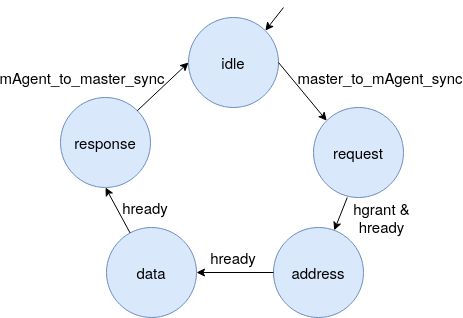
\includegraphics[width=5.5cm]{figs/hw/mAgent_FSM.png}
\caption{Master agent FSM}\label{fig:rafsm}
\end{wrapfigure}  

As seen from figure \ref{fig:rafsm} extra states are added to the system to enable the communication between the agent and the master. The agent will always be ready for a payload from the master, and when received it advances to the \textit{request\_phase}. At this point the agent has already translated and written the entire payload to the bus. In the \textit{request\_phase} \textbf{HBUSREQx} remains asserted until both \textbf{HGRANTx} and \textbf{HREADY} is set. When both signals are set the agent proceeds to the \textit{address\_phase} where it encodes \textit{nonsec} on its \textbf{HTRANS[1:0]} until \textbf{HREADY} is set. Otherwise \textbf{HTRANS[1:0]} will always be encoded with \textit{idle}. The agent proceeds to the \textit{data\_phase} where it waits until the \textbf{HREADY} is again set before sampling \textbf{HRDATA} and \textbf{HRESP}. It proceeds to the \textit{response\_phase} where it writes the payload to its master and returns to \textit{idle\_phase}. \\
\newline
The decision to write the entire payload to the bus already in the request phase stems from the property generation of the ESL. Instead of dividing this into a combination of blocking and shared ports updated in seperate cycles, reducing the level of abstraction significantly, it can safely be done as described so long as the encoding of \textbf{HTRANS[1:0]} is used in a correct manner. The only overhead is that it reduces throughput, but this is already reduced as a consequence of the blocking port combined with the need to report status back to the master. In a system with bursts implemented, the encoding of \textbf{HTRANS[1:0]} will also include \textit{seq}, but this feature is explored in chapter (ref something). Because of the decision to report status back to master in every transfer, the response data is sampled regardless of the transfer direction. This reduces ESL and verification complexity significantly, at the cost of one extra clock cycle latency for reads. 

\subsubsection{Slave agent}
Similarily to the master agent, only a subset of the AHB slave interface is written from the slave agent to the slave. This is the same payload as master agents. 

\begin{wrapfigure}{l}{5.5cm}
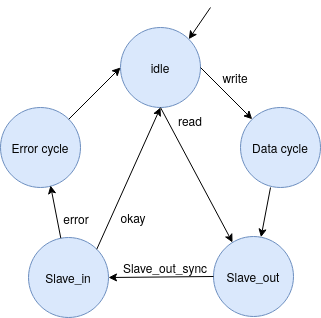
\includegraphics[width=5.5cm]{figs/hw/sAgent_FSM.png}
\caption{Master agent FSM}\label{fig:rsfsm}
\end{wrapfigure}  

As figure \ref{fig:rsfsm} shows the slave agent FSM is more complex than that of the master agent. To make the slave agent comply with the AHB protocol it needs to both obey the rules of the transfer phases and provide the proper response while communicating with its slave. In opposition to the master agent, a slave agent is not always ready to receive a payload from its master, namely the AHB matrix. Starting from the \textit{idle\_phase} the agent stays idle until it is both selected and the encoding of \textit{nonseq} is detected on its inputs. When true it samples address and control signals from the AHB matrix and proceeds to the \textit{data cycle} where it samples the data. After sampling the data, the payload is written to the slave out port named \textit{sAgent\_to\_slave}. At this point the agent waits for a handshake, which should normally occur instantly but that is not a requirement. After the handshake is received it proceeds to wait for the response data and status from the slave, as with the output there is not a strict requirement on the wait time but it is recommended to keep the wait states under 16 cycles in total. The slave agent deasserts \textbf{HREADY} throughout its entire conceptual data phase, and zeroes \textbf{HRDATA} one clock cycle after asserting \textbf{HREADY}. \\
\newline
The slave agent may at any given timepoint be operated by another master. This is why the slave deasserts its \textbf{HREADY} throughout its entire conceptual data phase. It is standard for a slave to introduce wait states. As with a DRAM module, there are delays associated with activating a row (insert data). As with DRAM this delay is minimized in sequental address transfers using bursts. In contrast to the diagram in figure \ref{fig:transfer}, the conceptual data phase of the slave agent does not include the assertion of \textbf{HREADY}. This is a slight misnomer since the data phase does infact include the assertion as seen from the properties. It is however not included in the FSM to not diffuse the differences between the states. The \textit{idle\_phase} and \textit{error cycle} only differentiate in the value of \textbf{HRESP}. Although the assertion of \textbf{HREADY} technically is a part of the data phase, it is however beneficial to highlight that these are seperate states, as they are represented as such in the RTL description. The zeroing of \textbf{HRDATA} is a design choice to increase abstraction. 
\newpage

\section{System level representation}
\label{sec:syslev}
\begin{figure}[hbt]
    \begin{center}
        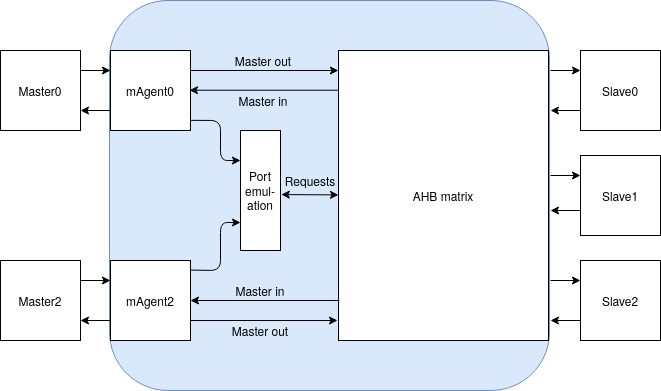
\includegraphics[width=0.8\textwidth]{figs/ESL/Syslev.png}
    \end{center}
    \caption{ESL toplevel with 2 masters and 3 slaves connected}
    \label{fig:esl_toplev}
\end{figure}
Representing an AHB design with an arbitrary number of masters and slaves on the systemlevel while simultaneously following the rules of SystemC-PPA is not straight forward. For a single master implementation it can be represented in a sequential manner, using only blocking ports. The generated properties are easy to refine in order to prove that the ESL description matches the hardware. When introducing a second master however, this representation becomes convoluted. Many different combinations of ports and methods were tried in order to try and both represent the hardware in simulation and have properties generated that would hold on the design. The main problem is the properties generated from the blocking ports transferring data from the masters to their agents. Due to the nature of the port it is only allowed for a single port to request a handshake in any given clock cycle. Trying to describe the hardware on the system level in this manner would require external arbitration, making the entire AHB architecture reduntant. For this reason it is necessary to split the design into clusters, which will be covered in more detail below. The choice falls naturally on having the master agents as seperate clusters. The GFV process was carried out on the remaining cluster to determine a feasible abstraction. 

 


\subsection{Proving completeness}
The first challenge of carrying out the GFV process is determining the CSM of the AHB. It has to be represented in such a way that it is feasible to describe at the ESL. It is necessary to know the state of the bus, namely if there is a transfer being carried out or not. It is not as simple as paying attention to bus ownership since there is no way of knowing if there is a transfer in progress when the default master owns the data bus, without looking at past values on \textbf{HTRANS[1:0]}. One would furthermore need to constrain the design to establish how far into the past to look. One could go with the suggested maximum delay of slaves for 16 clock cycles. A much simpler solution is to define the master agents states as outputs to their clusters, and define this as inputs to the main cluster. By only concerning with which masters are requesting and where the data goes, the CSM can be made quite simple. If one was concerned with which master owned the address and data bus it would lead to state explosion, making an ESL description unfeasible even for a low number of masters.     

\begin{figure}[ht!]
	\centering
	\begin{minipage}[t]{0.49\textwidth}
		\centering
		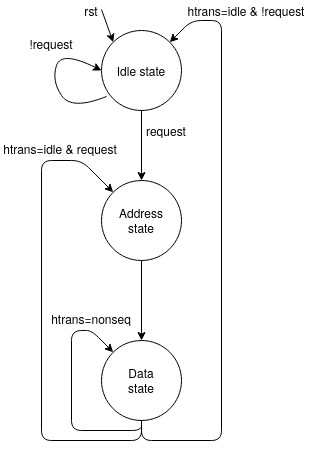
\includegraphics[scale=0.5]{figs/ESL/Bus_fsm_new.png}
		\captionof{figure}{Abstract CSM}
		\label{fig:OC}
	\end{minipage}
	\begin{minipage}[t]{0.49\textwidth}
		\centering
		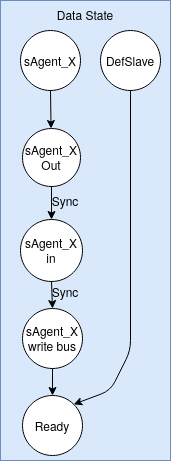
\includegraphics[scale=0.5]{figs/ESL/Data_state.png}
		\captionof{figure}{Detailed data state CSM}
		\label{fig:eslfsm}
	\end{minipage}
\end{figure}

By using a fixed priority arbitration scheme it is simple to determine which master is granted the bus. By dividing the transfer into three main states with the data state divided into five further, there is no need to impose any constraints on wait states. The bus is ready (\textbf{HREADY} is set) at the end of each state and any request is ignored unless the bus is ready. The states can be defined as follows:
\begin{itemize}
\item Idle state: No transfer in progress.
\item Address state: One master is in the address phase of the transfer, no masters are in the data phase. There is no trigger for the next state as the bus will always be ready here. 
\item Data state: One master is in the data phase of the transfer. This state has its own CSM based on which slave is being serviced.  
\end{itemize}

It is worth noting that in the idle and address state the bus is always ready. The payload is transferred between the states using visible register which are named \textit{AS\_regs} for the address state and \textit{DS\_regs} for the data state. The Data state is divided into several important states to describe the transaction between the slave and its agent while simultaneously describing all necessary outputs. The default slave has only two states and they are self explanatory because of the two cycle error response. The remaining slave agents are explained by the following:
\begin{itemize}
 \item First state: There is one clock cycle delay required to allow the slave agent time to sample the possible data provided in the data phase.
 \item Second state: Slave agent writes payload to slave using blocking write. 
 \item Third state: Slave agent reads back from slave using blocking read.
 \item Fourth state: Slave writes payload back to bus. This requires two cycles due to the possibility of error, error cycle was removed from master agent due to inconsistencies in simulation.  
 \item Fifth state: The bus is ready, payload is sampled, requests are handled and next state is determined based on the value of \textbf{HTRANS[1:0]}, which has been added to \textit{AS\_regs} alongside the payload. 
\end{itemize}

It is easy to see that the differentiation between read and write within the AHB matrix would lead to the double amount of data states, with the gain being one clock cycle saved in the case of a read. The entire design is represented by this CSM using only properties with length $t=1$ so determining the output is straightforward with the exception of \textbf{HGRANTx}. As this is an output that is not stored in a register its value updates in the same clock cycle as its instigator. This is not a problem to model in the properties themselves, but this representation does not allow for any sound abstraction between the RTL and ESL. Determining the value of \textbf{HGRANT} in the next clock cycle is not feasible in this implementation. One would have to account for every \textbf{HBUSREQx} as an assumption at $t+1$ in every property. An alternative could be to enable this output through a register but this would lead to unpredictable behaviour. This output is simply determined as the output of a function \textit{mx\_grant} and is at the ESL represented using an enum. \\
\newline
The design choice to zero \textbf{HRDATA} and modify the default slave response entails that \textbf{HRDATA} and \textbf{HRESP} will be zero unless it is in the fourth or fifth concepceptual data state. After adding all determination requirements and proving completeness the properties show that the interface between the master agents and AHB matrix cannot be represented using a single existing SystemC-PPA port. Referring back to section \ref{subsec:sysppa} there is a choice between three ports. Both the \textit{MasterSlave} and \textit{Shared} interface would result in the cycle accurate simulation of the design. Avoiding this is the main focus of this research. The representation of \textbf{HGRANTx} using cycle accurate values would also be necessary, which has already been established as infeasible. The remaining option is to emulate a single compound port using a combination of shared and blocking ports.          


\subsubsection{Combinatory port emulation}
When examining the FSM in figure \ref{fig:rafsm} it is seen that the traversal of the master agent state machine is always blocked by an input signal. The \textit{Request-}, \textit{Address-} and \textit{Data\_phase} are blocked by the AHB matrix's response signals \textbf{HREADY} and \textbf{HGRANTx}. Although the value of \textbf{HGRANTx} is impossible to determine effectively in the next clock cycle, its functionality with respect to the state machine can still be properly represented using a blocking port. The handshake from the master agents side represent the request, whereas the handshake from the AHB matrix side represent \textbf{HGRANTx} and \textbf{HREADY}. Due to the pipeline nature of the bus, a request can occur at any state of the bus as seen from figure \ref{fig:eslfsm}. This creates the requirement of a separate output representing \textbf{HREADY} alone, to allow for state machine traversal after bus has been granted. Referring to section \ref{subsec:sysppa} again, only one port read can be represented in each clock cycle for blocking ports. Due to each master agent requiring their own port for each of the cases, it is necessary to contain these ports in a seperate module, and treat it as a new type of port interface.
This port determines internally which master agent gets granted/unblocked with a simple fixed priority arbitration scheme. The final issue is having the port correctly represent updated requests. For this reason the port waits for a synchronization signal (handshake) from the AHB matrix. When this handshake is received the port peeks on all its request inputs and forwards this information to the AHB matrix through a \textit{Shared} interface, while simultaneously unblocking the highest priority requesting agent and every \textbf{HREADY} port that may be blocked. Special care has been taken to ensure that this happens in an atomic and synchronized manner. 
\newpage   
\begin{wrapfigure}{l}{5.5cm}
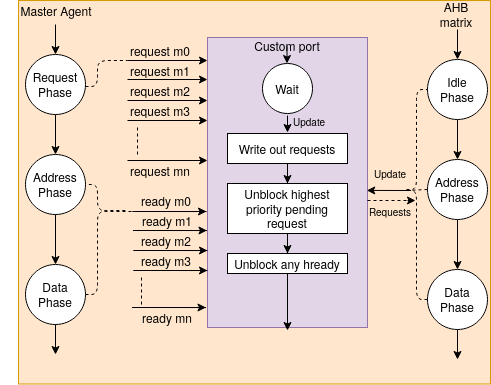
\includegraphics[width=5.5cm]{figs/ESL/port_diagram.png}
\caption{Illistration of port connection}\label{fig:cport}
\end{wrapfigure}

The port in figure \ref{fig:cport} is illustrated using the actual port directions in the ESL description, raher than the direction they symbolize. The inputs representing \textbf{HREADY} must be atomically unblocked which only happens when there is a pending handshake. To check for this the \textit{peek} function must be called, which is only available for reader ports. On the AHB matrix side the synchronization call to update the requests must always hand over control to the port by use of a wait function, which is only unconditionally called by use of a write port. When control is handed back to the AHB matrix the updated requests can be fetched from a shared port. 

\subsubsection{Master agent}

\subsubsection{Bus matrix}

\subsection{Refining properties}

\section{Simulation}
\label{sec:sim}

\subsection{Starvation}

\section{Generator}
\label{sec:generator}
